\documentclass[]{article}
\usepackage[hmargin=1in,vmargin= 1.4in]{geometry}
\usepackage{mathtools}
\usepackage{titling}
\usepackage{graphicx}
\usepackage{amsmath,amssymb,mathrsfs,wrapfig,setspace,gensymb,placeins,bm}
\usepackage[]{algorithm}
\usepackage{algorithmic}
\usepackage{verbatim}
\usepackage{subfigure}
\usepackage{caption}
\usepackage{lscape}
\usepackage{cite}
\usepackage{scrextend}
\usepackage{xcolor}
\usepackage{empheq}
\usepackage{tcolorbox}
\usepackage{amsthm}

\newcommand{\bmw}{\mbox{\boldmath $w$\unboldmath}}
\newcommand{\bma}{\mbox{\boldmath $a$\unboldmath}}
\newcommand{\bmA}{\mbox{\boldmath $A$\unboldmath}}
\newcommand{\bmb}{\mbox{\boldmath $b$\unboldmath}}
\newcommand{\bmr}{\mbox{\boldmath $r$\unboldmath}}
\newcommand{\bms}{\mbox{\boldmath $s$\unboldmath}}
\newcommand{\bmz}{\mbox{\boldmath $z$\unboldmath}}
\newcommand{\bmg}{\mbox{\boldmath $g$\unboldmath}}
\newcommand{\bmq}{\mbox{\boldmath $q$\unboldmath}}
\newcommand{\bmu}{\mbox{\boldmath $u$\unboldmath}}
\newcommand{\bmm}{\mbox{\boldmath $m$\unboldmath}}
\newcommand{\bmj}{\mbox{\boldmath $j$\unboldmath}}
\newcommand{\bmk}{\mbox{\boldmath $k$\unboldmath}}
\newcommand{\bmx}{\mbox{\boldmath $x$\unboldmath}}
\newcommand{\bmn}{\mbox{\boldmath $n$\unboldmath}}
\newcommand{\bmt}{\mbox{\boldmath $t$\unboldmath}}
\newcommand{\bmf}{\mbox{\boldmath $f$\unboldmath}}
\newcommand{\bmF}{\mbox{\boldmath $F$\unboldmath}}
\newcommand{\bmS}{\mbox{\boldmath $S$\unboldmath}}
\newcommand{\bmG}{\mbox{\boldmath $G$\unboldmath}}
\newcommand{\bmV}{\mbox{\boldmath $V$\unboldmath}}
\newcommand{\bmI}{\mbox{\boldmath $I$\unboldmath}}
\newcommand{\bmD}{\mbox{\boldmath $D$\unboldmath}}
\newcommand{\bmOmega}{\mbox{\boldmath $\Omega$\unboldmath}}
\newcommand{\bmtau}{\mbox{\boldmath $\tau$\unboldmath}}
\newcommand{\hyptan}{\mbox{tanh}}
\newcommand{\hypcos}{\mbox{cosh}}
\newcommand{\hypsin}{\mbox{sinh}}


\usepackage{titlesec}
\titleformat{\section}{\large\bfseries}{\thesection}{1em}{}
\renewcommand\thesection{\Roman{section}}

\setlength{\droptitle}{-10em}
\title{An Eulerian-Lagrangian method for simulating the interaction of a 
 Non-Newtonian fluid with complex shaped micro-swimmers}
\author{B. Vargas-Torres,
   T. Solano, Y. Liu, K. Shoele, H. Mohammadigoushki, M. Sussman}

%% hexadecimal digits must be upper case.

\begin{document}
\maketitle
\vspace*{-10mm}
\section{Method} 
The numerical method used for the Eulerian part of
our micro-swimmer simulations is a staggered
grid, dynamic adaptive mesh refinement algorithm for 
incompressible multi-phase flow.  
The dynamics of the micro-swimmer geometry, represented on a 
Lagrangian grid, is coupled to the Eulerian fluid flow by way of converting
the Lagrangian representation of the micro-swimmer to a
Moment-of-Fluid Eulerian representation.  The details of the numerical 
method, excluding the staggered grid treatment for the 
non-Newtonian force terms,
are presented in the following journal articles: 
\cite{dyadechko2005moment,ArientiSussman2014,peihierarchical,OHTA201966}.

It is important to note that our results presented here
correspond to a staggered grid 
formulation which is known to have better stability properties than the
collocated formulation\cite{rhie1983numerical}.  
The source of the stability problems for a collocated grid algorithm
is that the pressure projection step corresponding
to the collocated formulation has a non-empty null space in the pattern of
a checkerboard velocity distribution.

The numerical algorithm
for simulating non-Newtonian multi-fluid/multi-phase flows that was
presented in \cite{OHTA201966} was for a collocated grid.  The numerical
algorithm presented in \cite{peihierarchical} was for a staggered grid,
but only Newtonian flows were simulated in \cite{peihierarchical}.
The non-Newtonian multi-fluid/multi-phase results presented in 
this report are distinct from \cite{OHTA201966}
in that the present results were computed on a staggered grid.

The potential pitfalls of the collocated formulation notwithstanding,
in Figures \ref{gasbubblecompare}, \ref{helix12p4}, and
\ref{helix47p5} below, it is observed that the collocated results of the
past agree, qualitatively, with the present staggered grid results.  This
is encouraging, since the present results (a) reinforce that the previous 
reported collocated results were ``reasonably valid'' and did 
not suffer from stability 
problems, and (b) reinforce that the present staggered grid method has 
been implemented ``reasonably correctly,'' and has a mathematical guarantee of 
stability\cite{GUITTET2015215} for future simulations.

The mathematical model governing our numerical method is given as follows:
\begin{eqnarray}
	\nabla\cdot\vec{u}=0 \label{divfree}
\end{eqnarray}
\begin{eqnarray}
	\frac{\partial(\rho\vec{u})}{\partial t}+
	\nabla\cdot(\rho\vec{u}\vec{u}^{T})=
	\nabla\cdot(-p\bmI + \bmtau) \label{momentum}
\end{eqnarray}
\begin{eqnarray}
\bmtau=\bmtau_{s}+\bmtau_{p} \label{solvent_and_polymer}
\end{eqnarray}
\begin{eqnarray}
\bmtau_{s}=2\mu_{s}\bmD=\mu_{s}(\nabla\vec{u}+\nabla\vec{u}^{T}) 
  \label{solvant_stress}
\end{eqnarray}
\begin{eqnarray}
\bmtau_{p}=\frac{\mu_{p}\bmf{s}(\bmA)}{\lambda}
	\label{polymer_stress}
\end{eqnarray}
\begin{eqnarray}
\overset{\triangledown}\bmA \equiv \frac{\partial\bmA}{\partial t} + 
  \nabla\cdot(\vec{u}\bmA)-
  \bmA\cdot\nabla\vec{u}-
  (\nabla\vec{u})^{T}\cdot\bmA=-\frac{f_{R}(\bmA)}{\lambda}
  \label{upper_convective_deriv}
\end{eqnarray}
\begin{eqnarray}
\frac{\partial\phi_{m}}{\partial t}+\vec{u}\cdot\nabla\phi_{m}=0
  \hspace{10pt} m=1,\ldots,M
\end{eqnarray}
$\vec{u}$ is the fluid velocity, $\rho$ is the density which can
have large jumps at material interfaces, $p$ is the pressure, and $\bmtau$
is a combination of the solvent stress tensor $\bmtau_{s}$ 
and polymer stress tensor, $\bmtau_{p}$.  $\mu_{s}$ is the solvent viscosity
which can have large jumps at material interfaces, $\bmD$ is the
rate of deformation tensor, $bmD=\nabla\vec{u}+\nabla\vec{u}^{T})$, 
and $\bmA$ is the configuration tensor. $\phi_{m}$ is the
level set function for material $m$ ($m=1,\ldots,M$) and
satisfies,
\begin{eqnarray}
	\phi_{m}(t,\vec{x})=\left\{ \begin{array}{cc}
	+d_{m} & \mbox{if $\vec{x}$ is in material $m$ at time $t$} \\
	-d_{m} & \mbox{if $\vec{x}$ is not in material $m$ at time $t$}.\\
\end{array}\right. \label{signeddist}
\end{eqnarray}
$d_{m}$ in (\ref{signeddist}) represents the closest distance from point 
$\vec{x}$ to the material $m$ interface.  The relaxation source term 
$f_{R}(\bmA)$ found in (\ref{upper_convective_deriv}) is defined as
follows
\begin{eqnarray}
	f_{R}(\bmA)=\left\{ \begin{array}{cc}
		\frac{\bmA}{1-\mbox{tr}(\bmA)/L^{2}}-\bmI &
		\mbox{FENE-P model} \\
		\frac{\bmA-\bmI}{1-\mbox{tr}(\bmA)/L^{2}} &
		                \mbox{FENE-CR model}
	\end{array}
	\right.
\end{eqnarray}
The polymer stress versus strain term $f_{s}(\bmA)$ found in
(\ref{polymer_stress}) is defined as follows
\begin{eqnarray}
	f_{s}(\bmA)=\left\{ \begin{array}{cc}
		\frac{\bmA}{1-\mbox{tr}(\bmA)/L^{2}}-\bmI &
		\mbox{FENE-P model} \\
		\frac{\bmA-\bmI}{1-\mbox{tr}(\bmA)/L^{2}} &
		                \mbox{FENE-CR model}
	\end{array}
	\right.
\end{eqnarray}
We refer the reader to the following references for more information on
the mathematical models for non-Newtonian 
fluids\cite{BIRD1980213,PURNODE19981}.

The (novel) results presented in this report are preliminary in that we only 
present results for the one-way coupling between the 
swimmer (prescribed Lagrangian description of its motion)
and the non-Newtonian fluid (Eulerian description of its motion).  The
prescribed swimmer motion influences the fluid motion but the fluid 
motion does not in turn effect the swimmer motion.  The swimmer (see
Figures \ref{helix12p4} and \ref{helix47p5}) undergoes 
rigid body motion in the form of
translation along the $z$ axis, $\vec{u}_{translate}=(0,0,w)$ and 
rotation about the $z$ axis $\vec{u}_{rotate}=(-\Omega y,\Omega x,0)$:
\begin{eqnarray}
	\frac{d\vec{x}_{swimmer}}{dt}= 
	\vec{u}_{translate}+\vec{u}_{rotate}.
\end{eqnarray}
The Eulerian fluid motion is coupled to the prescribed Lagrangian
swimmer motion by way of the no-slip condition,
\begin{eqnarray}
	\vec{u}_{fluid}(t,\vec{x})=
	\vec{u}_{translate}(\vec{x})+\vec{u}_{rotate},
\end{eqnarray}
which is satisfied by all points $\vec{x}$ on the swimmer surface at time
$t$.

\section{Results} 

Two types of results are presented in this report: (A) verification results, 
and (B) validation results.

\subsection{Verification Results: Rising gas bubble in non-Newtonian fluid}

In Figure \ref{gasbubblecompare} we compare computational results
for the rise of a gas bubble in a hybrid shear thinning and
FENE-CR liquid solution\cite{OHTA201966}.  The model parameters
for this test correspond to the parameters used in \cite{OHTA201966}
(see Figure 7 from \cite{OHTA201966}).  
The viscoelastic model is the hybrid
Shear thinning Carreau and FENE-CR model.  The specific non-Newtonian
model parameters are $n=1/2$, $L=10$, and $De=5$.
We expect to compute a bubble that attains
a very unique ``cusped-cap'' shape.

In our Figure \ref{gasbubblecompare}, we show the following 3 results:
(a) collocated results from \cite{OHTA201966},
(b) staggered quarter domain 3D results (mirrored across the $x-z$ and $y-z$ 
planes for comparison purposes) computed using our latest algorithm,
and 
(c) staggered 3D RZ (axisymmetric $R$-$Z$) results (revolved about the 
$z$ axis for comparison purposes).

With the latest staggered grid method, we are able to reproduce the cusped
cap shape that was computed with a collocated grid method.  
We remark that our new results are not in quantitative 
agreement with the previous collocated results, this can be attributed to 
either (a) not having enough data to compare at precisely the same
simulation time, or (b) a difference in treatment of the interface
jump conditions where a Newtonian gas meets with a Non-Newtonian 
liquid.

\begin{figure}[htpb]
\centering
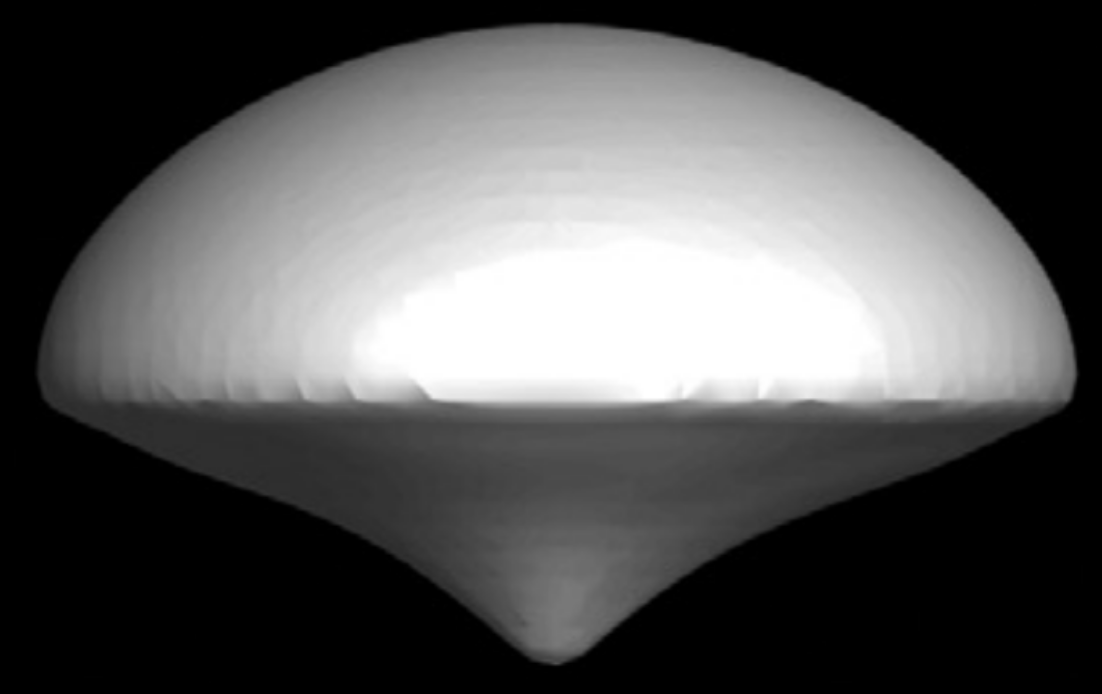
\includegraphics[width=0.3\textwidth]{collocated.png}
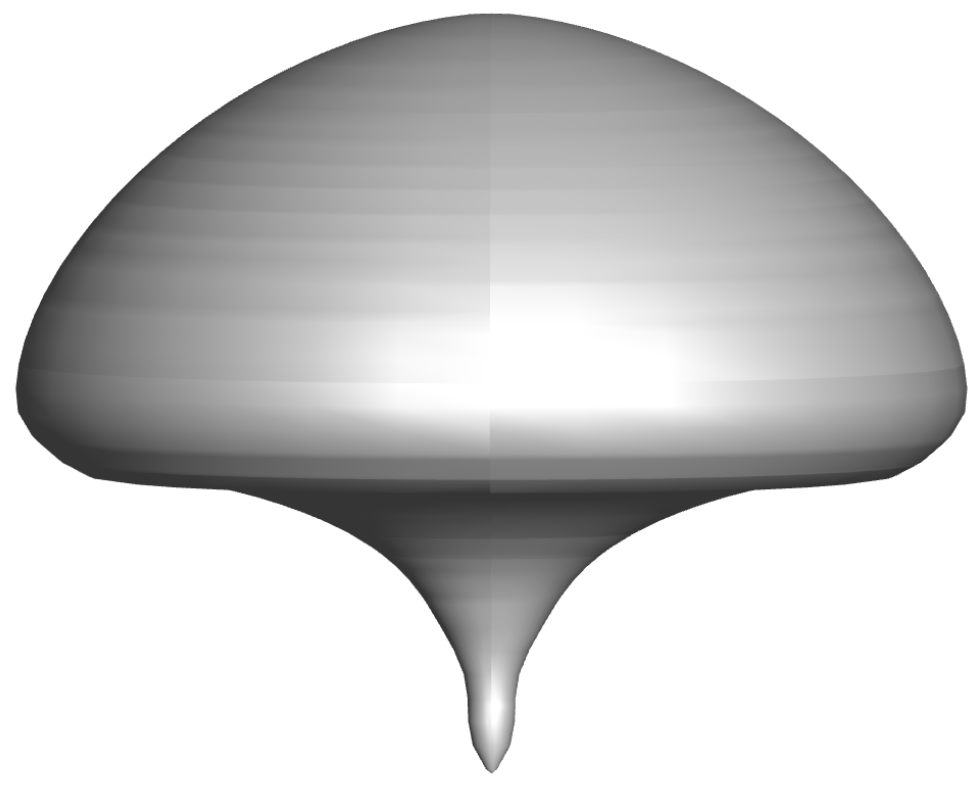
\includegraphics[width=0.3\textwidth]{staggared_rz_p434.png}
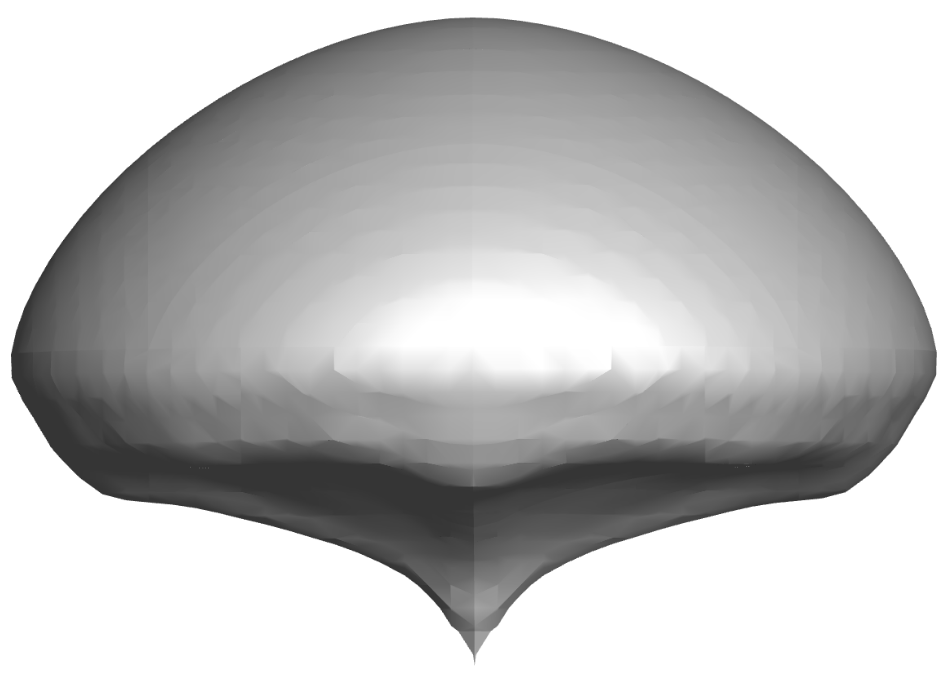
\includegraphics[width=0.3\textwidth]{staggared_qtr_p472.png}
\caption{Comparison between staggered and non-staggered algorithms for a
	gas bubble rising in a non-Newtonian fluid; from left to right:
	(a) collocated results 3D, (b) staggered results, 3D axi-symmetric,
	at time $t=0.434$, (c) staggered results, 3D, quarter domain simulation
	at time $t=0.472$. \label{gasbubblecompare} }
\end{figure}


\subsection{Validation Results and Discussion: 
 Helical swimmer in non-Newtonian fluid } 

%x=cos(omega t)  y=-sin(omega t)
%x'=omega y  y'=-omega x
% partial travels 2 pi radians in 2 pi/omega seconds i.e. omega radians/s
In Figures \ref{helix12p4} and \ref{helix47p5} we compare previous 
results for the $Q_{11}$ component of the configuration tensor
using the collocated algorithm with the current staggered
grid algorithm.  The pitch angle in Figure \ref{helix12p4} is 
$12.4$ degrees and the pitch angle in Figure \ref{helix47p5} is
$47.5$ degrees.  The liquid surrounding the swimmer is modeled as a 
FENE-P fluid.  The rotational velocity of the Helical swimmer for 
all of the simulations reported here is 
$\Omega=2\pi$ radians per second. 
The translational motion for both staggered grid
simulations was $0.00355$ cm/s.  Unfortunately, after the simulations
were completed, it was discovered that the translational motion for the
$12.4$ degrees collocated case was $0.015$ cm/s and the translational
motion for the $47.5$ degrees collocated case was $0.027$cm/s.

As is shown in the two comparison Figures, \ref{helix12p4} and
\ref{helix47p5}, we have qualitative agreement between the
previous collocated algorithm and the present staggered grid
algorithm.  Whereas the distribution of $Q_{11}$ is in agreement,
there is disagreement in the magnitude of $Q_{11}$.  We 
attribute this disagreement to the following:
(a) the translational velocity was different between the collocated
simulations and the staggered grid simulations, 
(b) the treatment of the boundary conditions where the non-Newtonian
liquid interacts with the dynamic helical swimmer is different
between the two formulations, and (c) (perhaps the biggest
reason for the difference) the recent staggered grid swimmer results
implemented more aggressive adaptive mesh refinement which has
the benefit of more efficient use of available computer resources,
but at the cost of less accuracy on the coarse parts of the 
computational domain.

\begin{figure}[htpb]
\centering
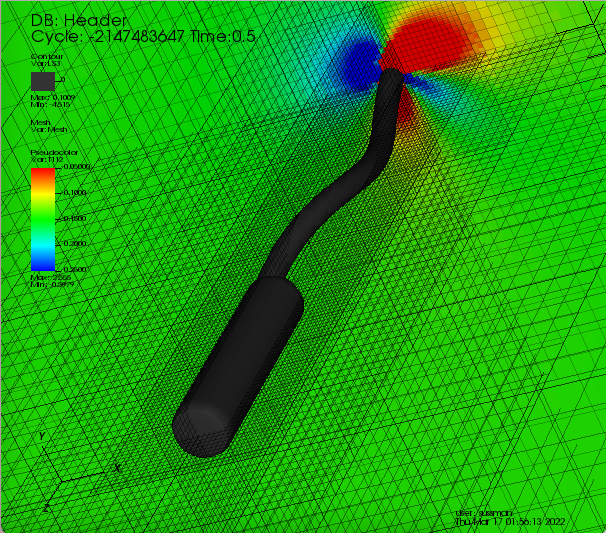
\includegraphics[width=0.4\textwidth]{collocated_12p4.png}
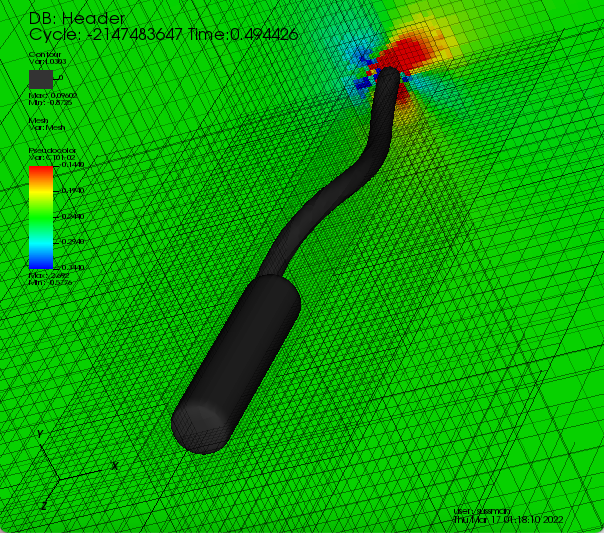
\includegraphics[width=0.4\textwidth]{staggared_12p4.png}
\caption{Comparison ($Q_{11}$ component) between staggered and 
    	non-staggered algorithms for 
        non-Newtonian FENE-P flow past a helical swimmer with pitch angle
        $12p4$ degrees.
	(a) left: collocated results, (b) right: staggered results,
	at time $t=0.5$. \label{helix12p4} }
\end{figure}

\begin{figure}[htpb]
\centering
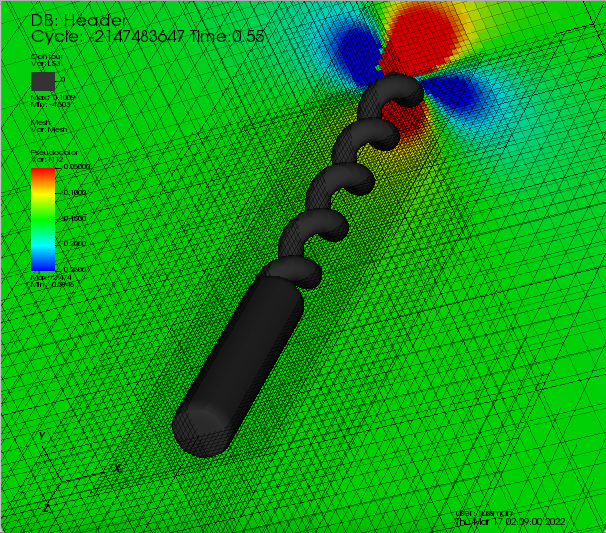
\includegraphics[width=0.4\textwidth]{collocated_47p5.png}
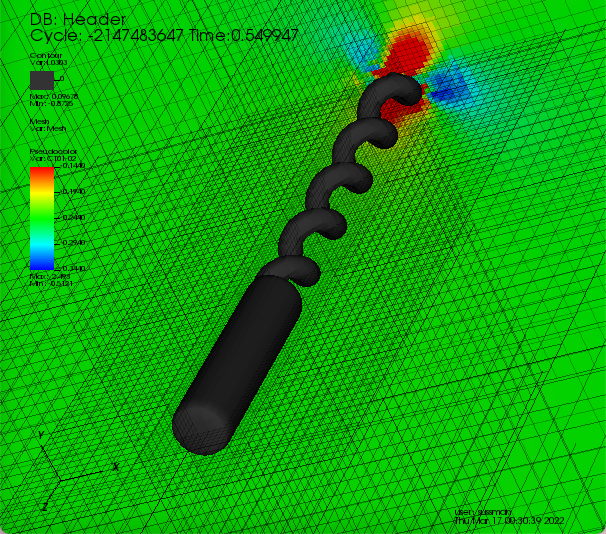
\includegraphics[width=0.4\textwidth]{staggared_47p5.png}
\caption{Comparison ($Q_{11}$ component) between staggered and 
    	non-staggered algorithms for 
        non-Newtonian FENE-P flow past a helical swimmer with pitch angle
        $47.5$ degrees.
	(a) left: collocated results, (b) right: staggered results,
	at time $t=0.55$. \label{helix47p5} }
\end{figure}

\section{Conclusions} 

A new staggered grid numerical method has been developed for simulating
the Eulerian-Lagrangian interaction of a ``Helical Micro-swimmer'' with
the surrounding Non-Newtonian fluid.
In comparing the present (novel) staggered grid numerical method for
non-Newtonian multi-phase, multi-fluid flow with the previous 
collocated grid results, we have observed qualitative agreement.  
In the results section above, we report on our reasonings for the
lack of quantitative agreement.  We believe the quantitative 
differences can be resolved in the future.
The staggered grid method is beneficial,
all things considered, because the method has inherent stability
properties\cite{GUITTET2015215} which will become important in 
the future when simulating
Eulerian-Lagrangian interaction phenomena with more energetic
forcing terms.  Also it is planned for the future to include
fluctuating hydrodynamics 
modeling\cite{PLUNKETT2014121,wang2018fluctuating} 
into our simulations.

\newpage
\bibliographystyle{acm}
\bibliography{references}

\end{document}

